
\chapter{Содержание}

\textit{Цель работы}: построение гистограммы и эмпирической функции распределения.
\begin{itemize}
	\item Для выборки объема n из генеральной совокупности X реализовать в виде программы на ЭВМ:
	\begin{enumerate}
		\item вычисление максимального значения $M_{max}$ и минимального значения $M_{min}$;
		\item размаха $R$ выборки;
		\item вычисление оценок $\hat{\mu}$ и $S^2$ математического ожидания MX и дисперсии DX;
		\item группировку значений выборки в $m = [\log_2n] + 2$ интервала;
		\item построение на одной координатной плоскости гистограммы и графика функции плотности распределения вероятностей нормальной случайной величины с математическим ожиданием $\hat{\mu}$ и дисперсией $S^2$;
		\item построение на другой координатной плоскости графика эмпирической функции распределения и функции распределения нормальной случайной величины с математическим ожиданием $\hat{\mu}$ и дисперсией $S^2$.
	\end{enumerate}
	\item Провести вычисления и построить графики для выборки из индивидуального варианта.
\end{itemize}


\chapter{Теория}
Пусть $\vec{x} = (x_1, \dots x_n)$ -- выборка из генеральной совокупности $X$ объема $n$.
\begin{enumerate}[wide=0pt]
	\item Максимальное значение выборки: $M_{max} = X_{(1)},$

	\item Минимальное значение выборки: $M_{min} = X_{(n)},$

	\item Размах выборки: $R = M_{max} - M_{min},$

	\item Оценка математического ожидания: $\hat{\mu}(\vec{X}) = \cfrac{1}{n}\sum_{i = 1}^{n}X_i,$

	\item Оценка дисперсии: $S^2(\vec{X}) = \cfrac{1}{n}\sum_{i = 1}^{n}(X_i - \bar{X})^2.$
\end{enumerate}


	$n(t, \vec{x})$ -- число компонент вектора $\vec{x}$, которые меньше чем $t$. \textit{Эмпирической функцией распределения}, построенной по выборке $\vec{x}$ называется функция $F_n: \mathbb{R} \rightarrow \mathbb{R}$, определенная правилом \ref{pdf}.

\begin{equation}\label{pdf}
	F_n(t) = \cfrac{n(t, \vec{x})}{n}
\end{equation}

	\textit{Интервальный статистический ряд} --- это ряд $J = [x_{(i)}, x_{(n)}]$, 
	который разбивают на $m$ промежутков, 
	ширина которых определяется согласно \ref{delta}:

	\begin{equation}\label{delta}
	\Delta = \cfrac{\left|J\right|}{m} = \cfrac{X_{(n)} - X_{(i)}}{m},
\end{equation}


\begin{equation}
	\begin{array}{ll}
		J_i = \left[x_{(1)} + \left(i - 1\right)\Delta; \; x_{(i)} + i\Delta\right), \; i = \overline{1,\: m - 1},\\
		J_m = \left[ x_{(1)} + \left(m - 1\Delta\right), \; x_{(n)}\right).
	\end{array}
\end{equation}

\textit{Эмпирической плотностью} распределения соответствующей выборке $\vec{x}$ называется функция \ref{cdf}:
\begin{equation}\label{cdf}
	f_n(x) = 
	\begin{cases}
		\cfrac{n_i}{n \cdot \Delta} & ,x \in J_i, \\
		0 & ,\text{иначе.}
	\end{cases}
\end{equation}

\chapter{Практика}

\begin{lstlisting}
function main()
	pkg load statistics

	X = dlmread("input.txt", ",");

	X = sort(X);
	% disp(X)

	% (a) минимальное и максимальное значение
	m_max = max(X);
	m_min = min(X);

	fprintf("(a) Максимальное значение выборки (M_max) = %f\n", m_max)
	fprintf("    Минимальное значение выборки  (M_min) = %f\n", m_min)
	fprintf("-------------------------------------------------\n")

	% (б) размах выборки
	r = m_max - m_min;
	fprintf("(б) Размах выборки (R) = %f\n", r)
	fprintf("------------------------------\n")

	% (в) вычисление оценок MX DX
	n = length(X)
	mu = sum(X) / n;
	s_2 = sum((X - mu).^2) / (n - 1);
	sigma = sqrt(s_2);

	fprintf("(в) Оценка математического ожидания (mu) = %f\n", mu)
	fprintf("    Оценка дисперсии (s_2) = %f\n", s_2)
	fprintf("----------------------------------------\n")

	% (г) группировка значений выборки в m = [log_2 n] + 2 интервала
	m = floor(log2(n)) + 2;

	bins = [];
	cur = m_min;

	for i = 1:(m + 1)
		bins(i) = cur;
		cur = cur + r / m;
	end

	eps = 1e-6;
	counts = [];
	j = 1;

	for i = 1:(m - 1)
		cur_count = 0;

		for j = 1:n

			if (bins(i) < X(j) || abs(bins(i) - X(j)) < eps) && X(j) < bins(i + 1)
				cur_count = cur_count + 1;
			endif

		endfor

		counts(i) = cur_count;
	endfor

	cur_count = 0;

	for j = 1:n

		if (bins(m) < X(j) || abs(bins(m) - X(j)) < eps) && (X(j) < bins(m + 1) || abs(bins(m + 1) - X(j)) < eps)
			cur_count = cur_count + 1;
		endif

	endfor

	counts(m) = cur_count;

	fprintf("(г) группировка значений выборки в m = [log_2 n] + 2 интервала:\n");

	for i = 1:(m - 1)
		fprintf("    [%f : %f) - %d вхожд.\n", bins(i), bins(i + 1), counts(i));
	end

	fprintf("    [%f : %f] - %d вхожд.\n", bins(m), bins(m + 1), counts(m));

	fprintf("----------------------------------------\n");

	% (д)  построение гистограммы и графика функции плотност

	fprintf("(д) построение гистограммы и графика функции плотности\n");
	fprintf("    распределения вероятностей нормальной случайной величины\n");

	figure;
	hold on;
	grid on;
	n = length(X);
	delta = r / m;
	middles = zeros(1, m);
	xx = zeros(1, m);

	for i = 1:m
		xx(i) = counts(i) / (n * delta);
	endfor

	for i = 1:m
		middles(i) = bins(i + 1) - (delta / 2);
	endfor

	fprintf("    высоты столбцов гистограммы:\n");

	for i = 1:m
		fprintf("    [%d] : %f\n", i, xx(i));
	endfor

	fprintf("[проверка] площадь гистограммы s = %f\n", sum(xx) * delta);

	set(gca, "xtick", bins);
	set(gca, "ytick", xx);
	set(gca, "xlim", [min(bins) - 1, max(bins) + 1]);
	bar(middles, xx, 1, "facecolor", "g", "edgecolor", "w");

	X_n = m_min:(sigma / 100):m_max;
	X_pdf = normpdf(X_n, mu, sigma);
	plot(X_n, X_pdf, "r");
	xlabel('X')
	ylabel('P')
	print -djpg hist.jpg
	hold off;

	fprintf("----------------------------------------\n");

	% (е) построение графика эмпирической функции распределения

	fprintf("(е) построение графика эмпирической функции распределения\n");
	fprintf("    и функции распределения нормальной случайной величины\n");

	figure;
	hold on;
	grid on;
	n = length(X);
	xx = zeros(1, length(X));
	curss = 1;

	bins = zeros(1, length(X));
	bins(1) = X(1);
	for i = 2:length(X)
		%fprintf("i = %d; curss = %d, X(I) = %d, xx = %d\n", i, curss, X(i), xx(curss))
		if (bins(curss) != X(i))
			curss+= 1;
			bins(curss) = X(i);
			xx(curss) = xx(curss-1);
		endif
		if (bins(curss) == X(i))
			xx(curss) += 1;
		endif
	end

	xx = xx ./ length(X);

	for i = curss:length(X)
		xx(i) = 1;
	end


	X_n = (min(X) - 0.5):(sigma / 100):(max(X) + 1.5);
	X_cdf = normcdf(X_n, mu, s_2);
	plot(X_n, X_cdf, "r");

	stairs(bins, xx);
	xlabel('X');
	ylabel('F');
	print -djpg cdf.jpg;
	hold off;
end

\end{lstlisting}



\chapter{Результаты}

\begin{figure}[ht!]
	\begin{center}
		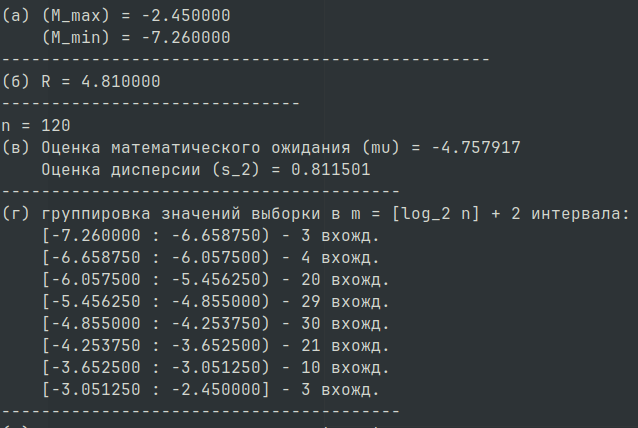
\includegraphics[scale=0.5]{assets/launch.png}
		\caption{Результат работы программы}
	\end{center}
\end{figure}

\begin{figure}[ht!]
	\begin{center}
		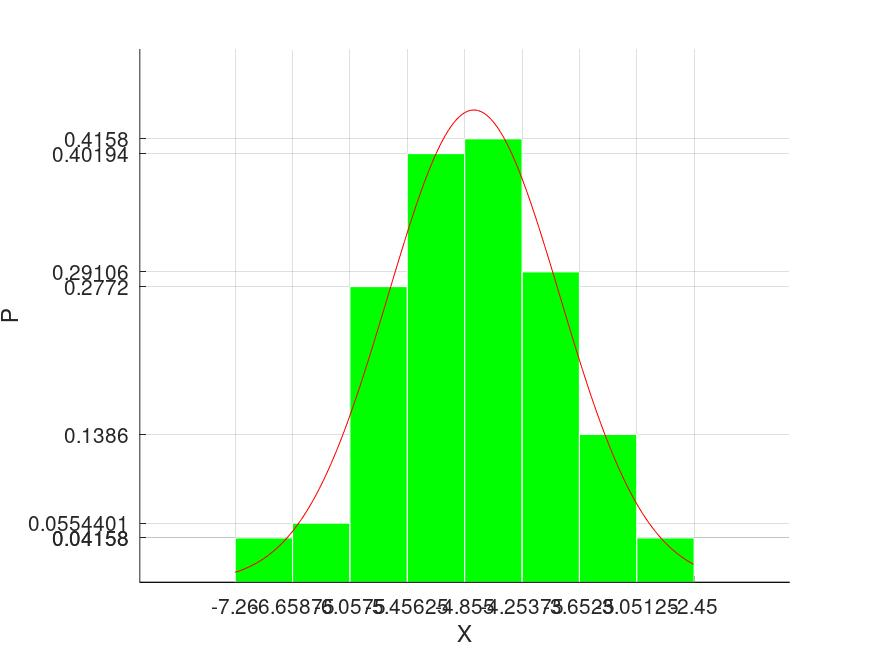
\includegraphics[scale=0.4]{assets/hist.jpg}
		\caption{Гистограмма и график функции плотности распределения вероятностей нормальной случайной величины}
	\end{center}
\end{figure}

\begin{figure}[ht!]
	\begin{center}
		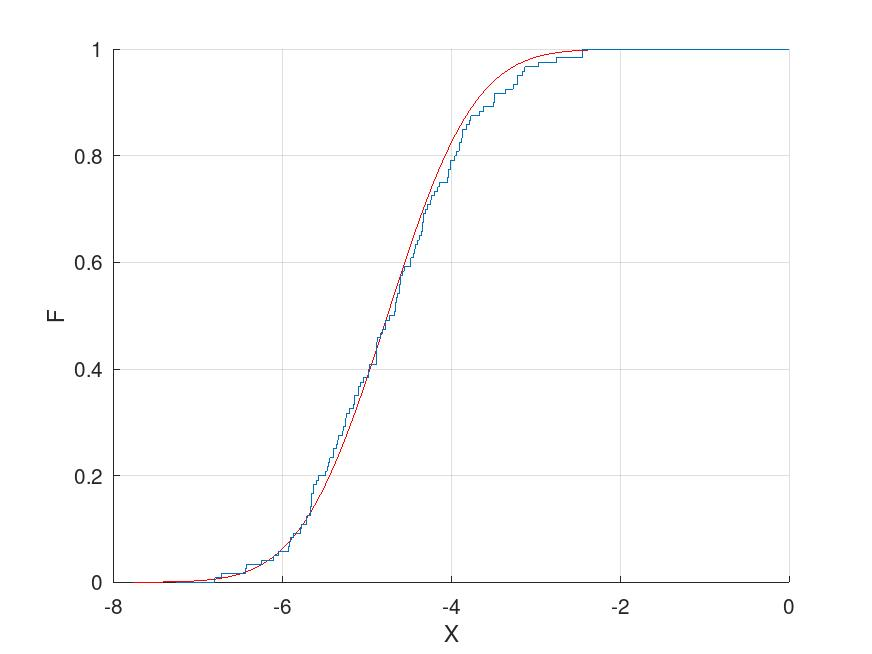
\includegraphics[scale=0.4]{assets/cdf.jpg}
		\caption{График эмпирической функции распределения и функции распределения нормальной случайной величины}
	\end{center}
\end{figure}